\chapter*{Dodatak: Prikaz aktivnosti grupe}
		\addcontentsline{toc}{chapter}{Dodatak: Prikaz aktivnosti grupe}
		
		\section*{Dnevnik sastajanja}
		
	%	\textbf{\textit{Kontinuirano osvježavanje}}\\
		
	%	 \textit{U ovom dijelu potrebno je redovito osvježavati dnevnik sastajanja prema predlošku.}
		
		\begin{packed_enum}
			\item  sastanak
			\item[] \begin{packed_item}
				\item Datum: 20. listopada 2022.
				\item Prisustvovali: Mario Petek, Ivan Kuzmić, Lovro Malojčić, Antonio Lukić, Ivan Kapusta, Eugen Preglej, Sven Leko
				\item Teme sastanka:
				\begin{packed_item}
					\item  sastanak s asistentom i demonstratorom
					\item  diskusija o radu na projektu
					\item  odabir tehnologije
				\end{packed_item}
			\end{packed_item}
			
			\item  sastanak
			\item[] \begin{packed_item}
				\item Datum: 23. listopada 2022.
				\item Prisustvovali: Mario Petek, Ivan Kuzmić, Lovro Malojčić, Antonio Lukić, Ivan Kapusta, Eugen Preglej, Sven Leko
				\item Teme sastanka:
				\begin{packed_item}
					\item  sastavljanje svih ekrana
					\item  općeniti izgled
				\end{packed_item}
			\end{packed_item}
		
			\item  sastanak
			\item[] \begin{packed_item}
				\item Datum: 27. listopada 2022.
				\item Prisustvovali: Mario Petek, Antonio Lukić, Lovro Malojčić
				\item Teme sastanka:
				\begin{packed_item}
					\item  sastanak s asistenticom
					\item  pojašnjenje zadatka
					\item  poboljšanje baze
				\end{packed_item}
			\end{packed_item}
		
			\item  sastanak
			\item[] \begin{packed_item}
				\item Datum: 12. studenoga 2022.
				\item Prisustvovali: Mario Petek, Ivan Kuzmić, Antonio Lukić, Ivan Kapusta, Eugen Preglej, Sven Leko, Lovro Malojčić
				\item Teme sastanka:
				\begin{packed_item}
					\item  pregled dosadašnjega rada
					\item  prijenos međusobnog znanja ostalim članovima
					\item  definiranje završnog rada za prvu verziju
				\end{packed_item}
			\end{packed_item}
		
			\item  sastanak
			\item[] \begin{packed_item}
				\item Datum: 17. studenoga 2022.
				\item Prisustvovali: Mario Petek, Ivan Kuzmić, Antonio Lukić, Ivan Kapusta, Eugen Preglej, Sven Leko, Lovro Malojčić
				\item Teme sastanka: 
				\begin{packed_item}
					\item  prezentiranje početne stranice
					\item  login
					\item  logout
					\item  deploy
				\end{packed_item}
			\end{packed_item}
		
			\item  sastanak
			\item[] \begin{packed_item}
				\item Datum: 05. prosinca 2022.
				\item Prisustvovali: Mario Petek, Ivan Kuzmić, Antonio Lukić, Ivan Kapusta, Eugen Preglej, Sven Leko, Lovro Malojčić
				\item Teme sastanka: 
				\begin{packed_item}
					\item  prvo kolokviranje
					\item  revizija napravljene aplikacije
				\end{packed_item}
			\end{packed_item}
		
			\item  sastanak
			\item[] \begin{packed_item}
				\item Datum: 22. prosinca 2022.
				\item Prisustvovali: Mario Petek, Ivan Kuzmić, Antonio Lukić, Ivan Kapusta, Eugen Preglej, Sven Leko, Lovro Malojčić
				\item Teme sastanka: 
				\begin{packed_item}
					\item  prezentacija alfa inačice aplikacije
					\item  dogovor za završnu verziju aplikacije
				\end{packed_item}
			\end{packed_item}
		
			\item  sastanak
			\item[] \begin{packed_item}
				\item Datum: 05. siječnja 2023.
				\item Prisustvovali: Antonio Lukić, Ivan Kapusta, Sven Leko
				\item Teme sastanka: 
				\begin{packed_item}
					\item  diskusija vezana oko basicAuth
					\item  rješavanje problema kod učitavanja i prikazivanja slike
				\end{packed_item}
			\end{packed_item}
			
			
		\end{packed_enum}
		
		\eject
		\section*{Tablica aktivnosti}

			\begin{longtblr}[
					label=none,
				]{
					vlines,hlines,
					width = \textwidth,
					colspec={X[7, l]X[1, c]X[1, c]X[1, c]X[1, c]X[1, c]X[1, c]X[1, c]}, 
					vline{1} = {1}{text=\clap{}},
					hline{1} = {1}{text=\clap{}},
					rowhead = 1,
				} 
				\multicolumn{1}{c|}{} & \multicolumn{1}{c|}{\rotatebox{90}{\textbf{Antonio Lukić}}} & \multicolumn{1}{c|}{\rotatebox{90}{\textbf{Ivan Kapusta }}} &	
				\multicolumn{1}{c|}{\rotatebox{90}{\textbf{Ivan Kuzmić }}} & 
				\multicolumn{1}{c|}{\rotatebox{90}{\textbf{Mario Petek }}} &	
				\multicolumn{1}{c|}{\rotatebox{90}{\textbf{Lovro Malojčić }}} & 
				\multicolumn{1}{c|}{\rotatebox{90}{\textbf{Sven Leko }}} &	
				\multicolumn{1}{c|}{\rotatebox{90}{\textbf{Eugen Preglej }}} \\  
				Upravljanje projektom 				& 15 & 2 & 2 & 2 & 2 & 2  & 2 \\ 
				Opis projektnog zadatka 			& 0 & 0 & 1 & 1 & 0 & 0 & 0 \\ 
				
				Funkcionalni zahtjevi       		& 0 & 0 & 3 & 3 & 0 & 0 & 0 \\ 
				Opis pojedinih obrazaca 			& 0 & 0 & 1 & 1 & 0 & 0 & 0 \\ 
				Dijagram obrazaca 					& 0 & 0 & 2 & 2 & 0 & 0 & 0 \\ 
				Sekvencijski dijagrami 				& 0.5 & 0 & 2 & 2 & 0 & 0 & 0 \\ 
				Opis ostalih zahtjeva 				& 0 & 0 & 0.5 & 0.5 & 0 & 0 & 0 \\ 

				Arhitektura i dizajn sustava	 	& 0 & 0 & 5 & 0 & 0 & 0 & 0 \\ 
				Baza podataka						& 0 & 0 & 5 & 4 & 0 & 0 & 0 \\ 
				Izrada baze podataka    			& 4 & 0 & 0 & 0 & 0 & 0 & 0 \\ 
				Dijagram razreda 					& 3 & 0 & 1 & 0 & 0 & 0 & 0  \\  
				Dnevnik sastajanja 					& 2 & 0 & 0.5 & 0.5 & 0 & 0 & 0 \\ 
				Popis literature 					& 0 & 0 & 1 & 1 & 0 & 0 & 0 \\
				Izrada početne stranice				& 0 & 0 & 0 & 0 & 0 & 0 & 15 \\  
				Spajanje s bazom podataka			& 0.5 & 3 & 0 & 0 & 0 & 3 & 0 \\  
				Setup back-enda 					& 5 & 2 & 0 & 2 & 5 & 2 & 0 \\  
				Setup front-enda 					& 0 & 1 & 0 & 0 & 8 & 1 & 8 \\  
				Deploy 								& 2 & 20 & 0 & 0 & 0 & 20 & 0 \\  
				Uploadanje slike 					& 5 & 10 & 0 & 0 & 0 & 10 & 0 \\ 
				Dijagram stanja						& 0 & 0 & 0 & 3 & 0 & 0 & 0 \\ 
				Dijagram aktivnosti					& 3 & 0 & 0 & 0 & 0 & 0 & 0 \\ 
				Dijagram komponenti					& 1 & 0 & 0 & 3 & 0 & 0 & 0 \\ 
				Korištene tehnologije i alati		& 0 & 0 & 0 & 2 & 0 & 0 & 0 \\ 
				Ispitivanje programskog rješenja	& 0 & 0 & 0 & 0 & 7 & 0 & 7 \\ 
				Dijagram razmještaja				& 0 & 2 & 0 & 0 & 0 & 0 & 0 \\ 
				Upute za puštanje u pogon			& 0 & 2 & 0 & 0 & 0 & 2 & 0 \\ 
				Zaključak i budući rad				& 0 & 0 & 0 & 4 & 0 & 0 & 0 \\ 
				  
				
			\end{longtblr}
					
					
		\eject
		\section*{Dijagrami pregleda promjena}
		
		\begin{figure}[H]
		\centering
		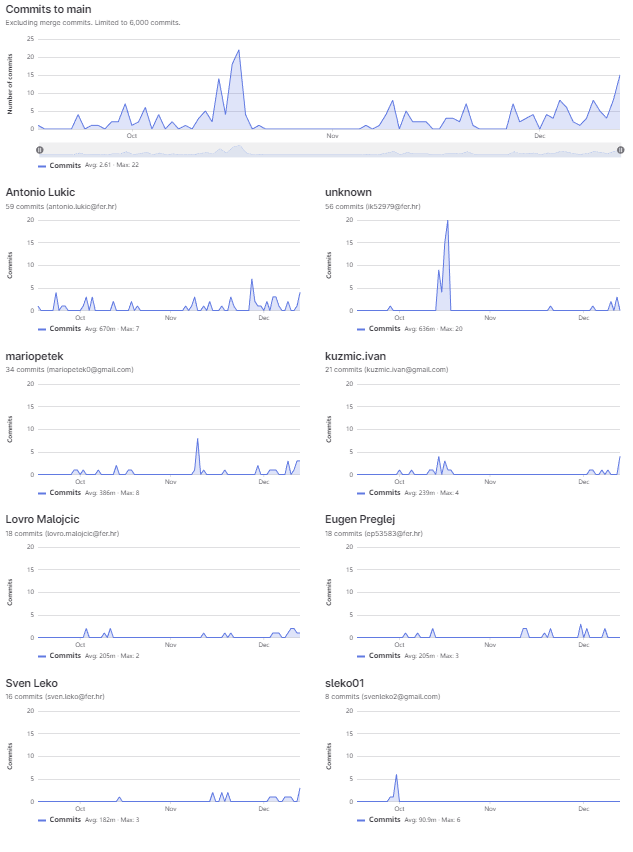
\includegraphics[width=14cm]{slike/dijagramPromjena}
		\caption{Dijagram pregleda promjena}
		\label{fig:Dijagram-promjena}
	\end{figure}
		
	